\tableofcontents

\newpage

\section{Задание}
По выданному преподавателем варианту восстановить текст заданного варианта программы и подпрограммы (программного комплекса), определить предназначение и составить его описание, определить область представления и область допустимых значений исходных данных и результата, выполнить трассировку программного комплекса.

\begin{figure}[H]
\centering

\includegraphics[scale=0.6]{task}
\label{pic:task}
\end{figure}


\section{Текст программы}
\subsection{Основная программа}
\begin{center}
		\begin{tabular}{|c|c|c|l|}
			\hline
			\multicolumn{1}{|c}{\makecell{\textbf{Адрес}\\\textbf{ячейки}}}
			&\multicolumn{1}{|c|}{\makecell{\textbf{Содержимое}\\\textbf{ячейки}}}
			&\multicolumn{1}{|c|}{\makecell{\textbf{Мнемоника}}}
			&\multicolumn{1}{c|}{\makecell{\textbf{Комментарии}}}\\
			\hline
			39C & 0200 & CLA & Очистка аккумулятора \\

			39D & EE19 & ST IP + 25 & Сохраненине 0 в ячейку 0x3B7 \\
			\hline
			39E & AE16 & LD IP + 22 & Загрузка в AC содержимого из ячейки 0x3B5 \\

			39F & 0C00 & PUSH & Запись AC в стек \\

			3A0 & D6FF & CALL 6FF & Вызов подпрограммы по адресу 0x6FF \\

			3A1 & 0800 & POP & Чтение из стека в AC \\

			3A2 & 6E14 & SUB IP + 20 & Вычитание из AC содержимого ячейки 0x3B7 \\

			3A3 & EE13 & ST IP + 19 & Сохраненине AC в ячейку 0x3B7 \\

			\hline
			3A4 & AE0F & ST IP + 15 & Загрузка в AC содержимого из ячейки 0x3B4 \\

			3A5 & 0740 & DEC & Декремент AC\\

			3A6 & 0C00 & PUSH & Запись AC в стек\\

			3A7 & D6FF & CALL 6FF & Вызов подпрограммы по адресу 0x6FF\\

			3A8 & 0800 & POP & Чтение из стека в AC\\

			3A9 & 4E0D & SUB IP + 13 & Вычитание из AC содержимого ячейки 0x3B7 \\

			3AA & EE0C & ST IP + 12 & Сохраненине AC в ячейку 0x3B7 \\
			\hline
			3AB & AE0A & LD IP + 10 & Загрузка в AC содержимого ячейки 0x3B6 \\

			3AC & 0700 & INC & Инкремент AC \\

			3AD & 0C00 & PUSH & Запись AC в стек \\

			3AE & D6FF & CALL 6FF & Вызов подпрограммы по адресу 0x6FF\\
			3AF & 0800 & POP & Чтение из стека в AC \\

			3B0 & 0740 & DEC & Декремент AC \\

			3B1 & 4E05 & SUB IP + 5 & Вычитание из AC содержимого ячейки 0x3B7 \\

			3B2 & EE04 & ST IP + 4 & Сохранение AC в ячейку 0x3B7 \\

			3B3 & 0100 & HLT & Остановка ТГ \\
			\hline
			3B4 & ZZZZ & Z & Переменная \\

			3B5 & YYYY & Y & Переменная \\

			3B6 & XXXX & X & Переменная \\

			3B7 & 0D08 & R & Результат \\
			\hline
	\end{tabular}
\end{center}

\newpage




\subsection{Подпрограмма}
\begin{center}
	\begin{tabular}{|c|c|c|l|}
		\hline
		\multicolumn{1}{|c}{\makecell{\textbf{Адрес}\\\textbf{ячейки}}}
		&\multicolumn{1}{|c|}{\makecell{\textbf{Содержимое}\\\textbf{ячейки}}}
		&\multicolumn{1}{|c|}{\makecell{\textbf{Мнемоника}}}
		&\multicolumn{1}{c|}{\makecell{\textbf{Комментарии}}}\\
		\hline
		6FF & AC01 & LD \&1 & Чтение из стека входного параметра \\

		700 & F207 & BMI IP + 7 & Если значение параметра меньше нуля, то\\ & & & переход в ячейку 0x708 \\
		701 & 7E09 & CMP IP + 9 & Сравнение AC с содержимым ячейки 0x70B \\

		702 & F905 & BGE IP + 5 & Если значение параметра больше или равно, то\\ & & & переход в ячейку 0x708 \\

		703 & 0500 & ASL & Арифметический сдвиг влево \\

		704 & 0500 & ASL & Арифметический сдвиг влево \\

		705 & 4C01 & ADD \&1 & Сложение входного параметра с AC \\

		706 & 4E05 & ADD IP + 5 & Сложение сожержимого ячейки 0x70C с AC \\
		707 & CE01 & BR IP + 1 & Безусловный переход в ячейку 0x709 \\

		708 & AE02 & LD IP + 2 & Загрузка в AC содержимого ячейки 0x70B\\
		709 & EC01 & ST \&1 & Сохранение AC на место входного параметра в стеке \\
		70A & 0A00 & RET & Возврат из подпрограммы \\
		\hline
		70B & 0B10 & a & Локальная переменная \\

		70C & 00FA & b & Локальная переменная \\
		\hline	
	\end{tabular}
\end{center}

\section{Описание программы}
\subsection{Назначение программы и реализуемая ею функция}
\subsubsection{Реализуемая программой функция}
	\begin{center}
		$ R = F(Y) - F(Z-1) - F(X+1) + 1 $
	\end{center}
\subsubsection{Реализуемая подпрограммой функция}
	\begin{center}
		\[
			F(x) =  \begin{cases}
			a & \textrm{, для } x<0\textrm{,}\\
			a & \textrm{, для } x \geq a\textrm{,}\\
			5x + b & \textrm{, для } 0 \leq x < a\textrm{,}\\
			\end{cases}
		\]
	\end{center}

\subsubsection{График функции, реализуемый подпрограммой}
\begin{figure}[H]
	\centering
	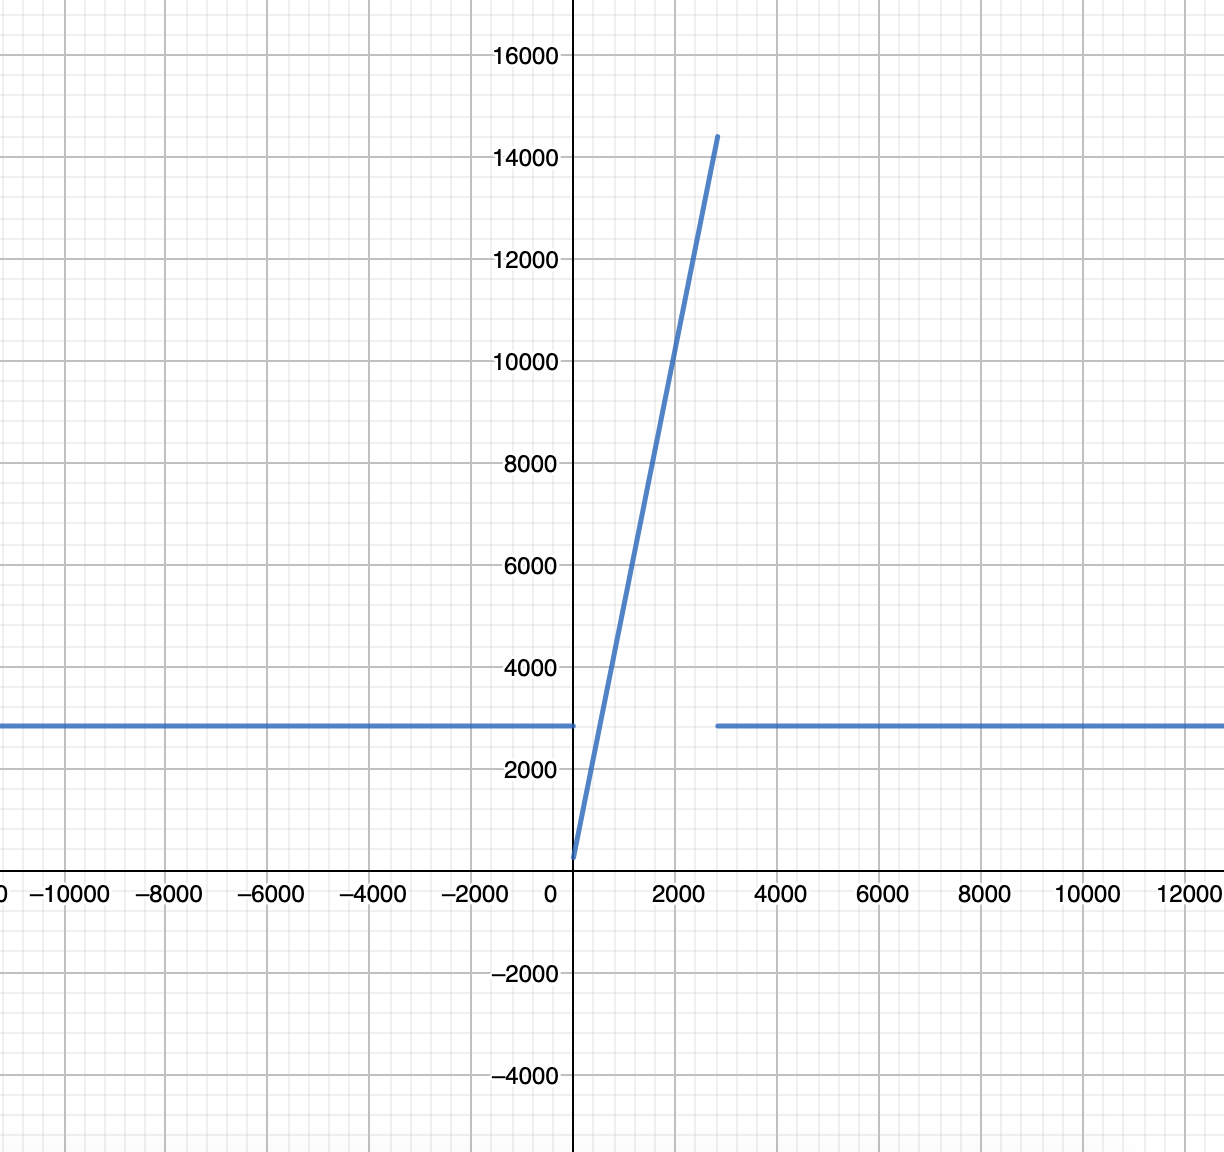
\includegraphics[scale=0.5]{grap}
	\label{pic:grap}
\end{figure}

\subsection{Область представления и область допустимых значений исходных данных и результата}
\subsubsection{Область представления}
\noindent Z, Y, X, R: 16-разрядные знаковые числа с фиксированной запятой. Диапазон значений формата: $-2^{15}\ldots2^{15}-1$\\


\subsubsection{Область допустимых значений}
\noindent Область допустимых значений R: $-2^{15}\ldots2^{15}-1$\\
\\
Область допустимых значений входного аргумента подпрограммы (т.е. $ X,Y,Z $):\\
\hspace*{1cm} Пусть $ F(x) $ - реализуемая подпрограммой функция, тогда ОДЗ для нее будет $-2^{15}\ldots2^{15}-1$.\\
\\
\hspace*{1cm} 1) Пусть $ -32768 \leq x<0 $, тогда $ F(x) = a $
\\
\hspace*{1cm} 2) Пусть $ a \leq x \leq 32767 $, тогда $ F(x) = a $
\\
\hspace*{1cm} 2) Пусть $ 0 \leq x < a $, тогда имеет место система:
\[
	\begin{cases}
	-32768 \leq F(x) \leq 32767\\
	-163 590\leq F(x)\leq 250\\
	\end{cases}
\]
\hspace*{1cm}Откуда $ F(x) = 5x + 250 \geq -32768 \Rightarrow x \geq -6604$\\
\hspace*{1cm}В итоге \[
	\begin{cases}
	-6604 \leq x \leq 0\\
	-32768 \leq F(x) \leq 250
	\end{cases}
\]
\\

В итоге ОДЗ для $ X, Y, Z $ будет
\[
\begin{cases}
-6604 \leq x \leq 0 \\
x = 2832
\end{cases}
\]

\subsection{Расположение в памяти ЭВМ программы, исходных данных и результатов}
\subsubsection{Исходные данные и результат}
\noindent Z (0x3B4) - первый аргумент\\
Y (0x3B5) - второй аргумент\\
X (0x3B6) - третий аргумент\\
R (0x3B7) - результат выполнения программы\\
\subsubsection{Программа}
\noindent 0x39C --- 0x3B3 - основная программа\\
0x6FF --- 0x70A - подпрограмма\\
a (0x70B), b (0x70C) - локальные переменные, используемые подпрограммой

\subsection{Адреса первой и последней выполняемой команд программы}
\noindent 0x39C - первая исполняемая команда программы\\
0x3B3 - последняя исполняемая команды программы\\

\newpage
\section{Таблица трассировки}
\begin{center}
	\begin{tabular}{|c|c|c|c|c|c|c|c|c|c|c|c|}
		\hline
		\multicolumn{2}{|c}{\makecell{\textbf{Выполняемая}\\\textbf{команда}}}
		&\multicolumn{8}{|c|}{\textbf{Содердимое регистров после выполнения команды}}
		&\multicolumn{2}{c|}{\makecell{\textbf{Ячейка, содержимое}\\\textbf{которой изменилось}}}\\
		\hline
		Адрес & Код & IP & CR & AR & DR & SP & BR & AC & NZVC & Адрес & Новый код\\
		\hline
	\end{tabular}
\end{center}
\newpage

\section{Вывод}
\noindent В ходе выполнения данной лабораторной работы я познакомился с реализаций стека в БЭВМ. Также я научился работать с подпрограммами и узнал какими способами можно передавать аргументы в подпрограммы.